\begin{sectionblock}{Goals}
  Finding online resources for college
  mathematics is not difficult.

  \vspace{1ex}
  But finding resources that are readily available, field-tested in a
  variety of settings, and known to be high quality is a
  challenge. \textbf{This project will\ldots}
  \begin{enumerate}
  \item provide materials like textbook
    content, videos, interactive applets, and instructor guides;\\[1ex]
    \begin{center}
      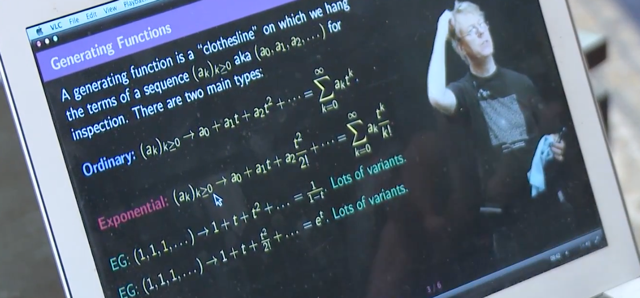
\includegraphics[width=0.65\textwidth]{tom.png}
    \end{center}
  \item identify best practices for building comprehensive,
    quality-controlled, and curated libraries of freely reusable
    instructional materials for college-level mathematics courses;
  \item investigate the impact of such a library on faculty adoption of
    evidence-based teaching practices.
  \end{enumerate}
\end{sectionblock}


